\begin{htmlonly}
\documentclass{covise}

\usepackage{html, htmllist}
\usepackage{color}
\usepackage{graphicx}
\usepackage{longtable}
\usepackage{palatino}
\usepackage{picins}
\usepackage[colorlinks,dvips]{hyperref}
	  
\bodytext{TEXT=#000000 BGCOLOR=#FFFFFF LINK=#0033CC VLINK=#0033CC}

% #1  mark defined by \label
% #2  a linktext 
% #3  a html link 
\newenvironment{covlink}[3]%
{\html{\htmladdnormallink{#1}{#3}}\latex{\hyperref[#1]{#2} (\ref{#1})}%
}

\newenvironment{covimg}[4]%
{ \html{\htmladdimg[ALIGN=CENTER]{#2.gif}}
 
 \latexonly
 \begin{figure}[!Hhtp]
  \begin{center}
   \includegraphics[scale=#4]{#1/#2}
   \caption{#3}
  \end{center}
 \end{figure}
 \endlatexonly
}



\definecolor{output}{rgb}{0.,0.,1.}
\definecolor{depend}{rgb}{1.,0.65,0.}
\definecolor{required}{rgb}{0.58,0.,0.83}
\definecolor{optional}{rgb}{0.,0.39,0.}

\end{htmlonly}

%================================================================================
%================================================================================


%================================================================================
%\startdocument

\chapter{Process Steps and Process Flow}

\begin{figure}[!Hhtp]
  \begin{center}
   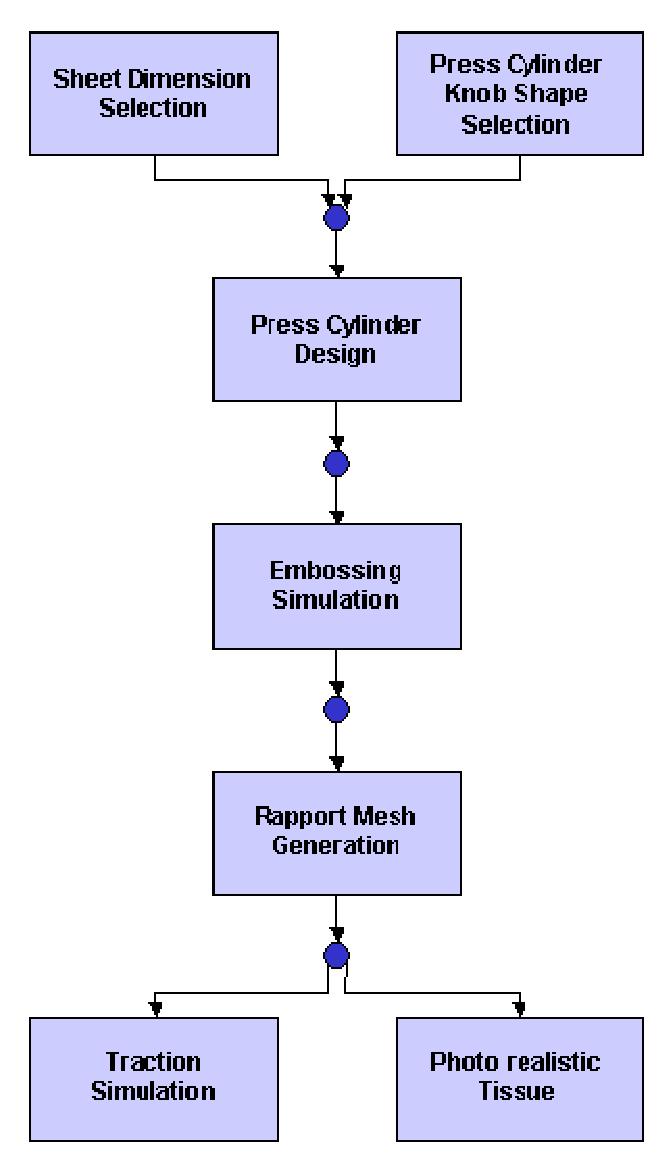
\includegraphics[scale=0.6]{process/flowchart_overview}
   \caption{Flowchart}
  \end{center}
\end{figure}

\section{Paper Size}

As a first step the user chooses the  paper size. There are three standard sizes for 
toilette paper (abbrev. toipa) and two standard sizes for household 
paper (abbrev. HHT). In addition, he has the possibility to customize 
a size of his own.

\vspace{0.5cm}
\begin{tabular}{|l|l|l|l|} \hline
Parameter 		& Type 		& Range 	& Unit	\\ \hline
fixed size 	& choice 	& Toipa 125x98	& $mm^2$ 	\\ 
				& 		 	& Toipa 140x98	&			\\
				& 		 	& Toipa 125x110	&			\\				
				& 			& HHT 246x260	& 			\\ 
			     	&			& HHT 246x230	& 			\\ 
				& 			& Custom Dimensions		& 			\\ \hline
variable length	& dial	& 100-300 		& $mm$ 		\\ \hline
variable width & dial	& 100-300 		& $mm$ 		\\ \hline
\end{tabular}
\vspace{0.5cm}

You can view the result of this process step as a threedimensional 
representation of the outline of the sheet.


\section{Knob Geometry of the Press Cylinder}

In the second step the user defines the geometry of single knobs on the press 
cylinder. The shape can be circular, elliptic, or rectangular, and it is 
defined by length, width, height, flank angle, abrasion radius, ground radius, and run-out zone.
The run-out zone is currently fixed to 1 mm. Length, width, height, flank angle, abrasion radius, 
and ground radius are parameters; in case of a circle specify length = width = diameter, 
for an ellipse specify length = major axis and width = minor axis. 


\begin{figure}[!Hhtp]
  \begin{center}
   \includegraphics[scale=0.7]{process/knob_new}
   \caption{Knob Geometry}
  \end{center}
\end{figure}

Since this knob geometry is used for embossing the tissue, and, therefore, 
a simulation may be required, the user should know beforehand whether simulation 
results are already available for his geometry in the data base.  
As a result of this search he gets a list of similar knobs from the data 
base, from which he can select the knob to be used in the following process. 
The criterion for 'similar' is first the shape of the knob, and second, 
for all knobs of this shape, a difference of not more than 10 \% in all 
other properties.

\vspace{0.5cm}
\begin{tabular}{|l|l|l|l|} \hline
Parameter 			& Type 		& Range 	& Unit	\\ \hline
Shape 				& choice 	& Circle, Ellipse, Rectangle			& 			\\ \hline
Length  	        & dial & 0.4-5.0		& $mm$ 		\\ \hline
Width	            	& dial & 0.4-5.0		& $mm$ 		\\ \hline
Height			& dial	& 100-300 	& $mm$ 	\\ \hline
Flank Angle		& dial	& 0.0-35.0 	& $\symbol{23}$ \\ \hline
Abrasion Radius	& dial	& 0.0-0.5 		& $mm$ 		\\ \hline
Ground Radius	& dial	& 0.0-0.5 		& $mm$ 		\\ \hline
Data Base 		& choice	& see below   &			\\ \hline
\end{tabular}
\vspace{0.5cm}

The list of similar knobs may look different each time; this is an example:
\begin{itemize}
\item my knob (not) in DB (h=2.0 l=0.4 b=0.4 a=20 ra=0.5 rg=0.5)
\item similar knob in DB (h=2.0 l=0.4 b=0.4 a=20 ra=0.5 rg=0.5)
\item similar knob in DB (h=2.0 l=0.4 b=0.4 a=20 ra=0.5 rg=0.5)
\end{itemize}

If the user chooses a knob other than the one selected via parameters, the parameters are 
adapted automatically.

The visible result of this process step is a threedimensional representation of the knob, 
made up of a few polygons.


\section{Design of the Embossing Pattern}

In the third step the user decides about the pattern. There are two possibilities: 
parametric or free design of the pattern. In both cases the positions of the 
knobs in the repeating pattern are defined by this step.

The visible result of this process step is a threedimensional representation of the pattern 
on a sheet. The repeating pattern is replicated as often as needed to fill 
in the sheet. The representation of the knob is taken from the geometry of 
a knob on the cylinder; i.e. the user sees a winding off of the cylinder on a sheet.

During design there is a permanent test whether this design allows a simulation 
of  traction later on. For a simulation the single knobs have to be combined 
to form a complete mesh later on.
But this will only work if the knobs including their run-out zone are not 
too close together or even intersect {\it (criterion for 'too near': runout
zones of 2 knobs intersect)}.   
Therefore, in addition, the representation contains  the outline of the bottom 
of the knob. The outline is shown in blue as long as the design is feasible, 
it becomes yellow if  knobs are getting too close.


\subsection{Parametric Design}

'Parametric' means that the pattern is defined by a couple of parameters. 
Thus you can easily generate some simple basic embossings, where the knobs 
are placed along a straight line. The user specifies the angle between the straight 
line and the edge, and the distance between knobs on the straight line. 
In case of parametric design the repeating pattern adapts itself automatically, 
so that it contains a quarter of  two adjacent knobs on a straight line 
respectively. The complete pattern is generated by replicating (relocating) 
the repeating pattern. The orientation of the repeating pattern remains unchanged.

 
\begin{figure}[!Hhtp]
  \begin{center}
   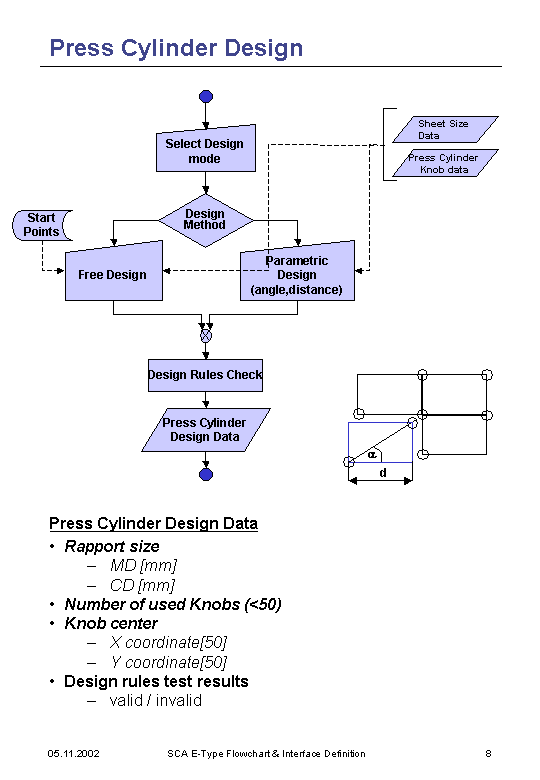
\includegraphics[scale=0.7]{process/pdesign}
   \caption{Parametric Design}
  \end{center}
\end{figure}

\vspace{0.5cm}
\begin{tabular}{|l|l|l|l|} \hline
Parameter 		& Type 		& Range 	& Unit		\\ \hline
angle			& dial	& 0.0-90.0 		& \symbol{23}	\\ \hline
distance 		& dial	& 10.0-0.7 		& $mm$ 			\\ \hline
\end{tabular}
\vspace{0.5cm}

\subsection{Free Design}
Free design means that the user can read in the positions of the knobs from a 
file, and then change them interactively.  He is free to choose length and 
width of the repeating pattern. Thus he can generate complex patterns.


\begin{figure}[!Hhtp]
  \begin{center}
   \includegraphics[scale=0.7]{process/fdesign_new}
   \caption{Free Design}
  \end{center}
\end{figure}


The file is in ascii format and looks as follows:
\begin{samepage}
\begin{verbatim}
20.0 20.0

11

 8.0  0.0
 5.0  5.0
 0.0  8.0
20.0  0.0
15.0  5.0
10.0 10.0
 5.0 15.0
 0.0 20.0
20.0 12.0
15.0 15.0
12.0 20.0
\end{verbatim}
\end{samepage}

The first row contains the size of the repeating pattern in mm, 
the second one the number of points, and the following rows contains 
the x- and y- coordinates of the points based on the bottom left 
corner of the repeating pattern. 


\vspace{0.5cm}
\begin{tabular}{|l|l|l|l|} \hline
Parameter 		& Type 		& Range 	& Unit		\\ \hline
Rapport Length		& dial	& see below	& $mm$			\\ \hline
Rapport Width	 	& dial	& see below	& $mm$ 			\\ \hline
\end{tabular}
\vspace{0.5cm}

The range of allowable values for rapport length and width is taken from the
COVISE map used for the visualization process. Currently a range of 2-20 or
2-30 is used but you may have to modify these values after you have gained more
experience.\newline
\newline
Please note: 
\begin{itemize}
\item The user interface (COVER) allows you to specify
values in the range given by the COVISE map. 
\item To extend this range you have to
modify the map (see chapter 3.10 - ControlSCA module).
\end{itemize}  
The interactive change of the positions of the knobs is implemented as 
direct manipulation, i.e. the user selects the knob using the threedimensional 
input value and moves it.


\section{Simulation of Embossing}

In the real embossing process the tissue is placed on a rubber support, and 
is embossed using a metal cylinder. The simulation will compute the deformation 
in all these three areas (rubber, tissue, metal). The numerical simulation works 
as follows: First, decompose the areas for which the deformation will be computed 
into cells, and then solve the deformation equations for these cells. This 
decomposition into cells is called grid generation, and this process is difficult 
to automize, because you have to adapt the size of the cells to the expected 
deformation (you can use large cells for areas with minor deformation, and you 
need smaller cells only for areas with strong deformation). The grid contains 
significantly more cells than the geometry (which is needed for the representation 
of the design).  In addition, the shape of the cells affects the quality of the 
results of the computation; the cells should have not too acute angles. The 
geometry of knobs is, however, based on rectangular and elliptic knobs, and 
the problem areas are therefore well known; thus an automatic grid generator 
could be developed in the frame of this projects.

The tissue and the metallic part (of  the quarter of a knob) are decomposed into 
twodimensional cells, the rubber - because it is subject to strong 
deformation - has to be decomposed into threedimensional cells.

Then the user has to select the tissue material; he can choose from six 
materials. In addition, he has to adjust the contact pressure and the hardness 
of the rubber.

This data are used to generate the input file for the simulation. But now the 
real simulation of the embossing can be started using the LS-Dyna program. 
The result of the simulation contains the grid of the deformed tissue for 
one knob and tensions resp. deformation in the cells of the grid.

Since grid generation and simulation take a lot of time the results are stored into 
a data base. Therefore, after the user has selected type of tissue, hardness of 
rubber, and contact pressure, the program tests if there are simulation results 
for these or similar parameters, and provides them as a list. If the user decides 
to use parameters from the data base, no real simulation is started at all but 
the results are taken from the data base. 

\vspace{0.5cm}
\begin{tabular}{|l|l|l|l|} \hline
Parameter 		& Type 		& Range 	& Unit	         \\ \hline
Rubber Hardness  	& dial		& see Note 1 	& \symbol{23} $Shore$ \\ \hline
Contact Pressure	& dial		& see Note 2 	& $N per knob$ 	 \\ \hline
Tissue Type      	& Choice 	& TAD		&		 \\ 
			& 		& Slush 	&		 \\
			& 		& Double Velvet &		 \\				
			& 		& HHT Convent	& 		 \\ 
			&		& HHT      	& 		 \\ 
			& 		& BSQ A 	& 		 \\ \hline
Data Base		& choice	& see Note 3	& - 		 \\ \hline
Start Embossing     	& Boolean   	& -             & -              \\ \hline
\end{tabular}
\vspace{0.5cm}


Please note: 
\begin{enumerate}

\item Currently the value for Rubber Hardness is ignored (except that it is stored in the database), 
and simulation starts with predefined values.

\item Contact Pressure actually meens the maximum force applied {\bf per knob}. This value
can be modified within a range defined in the map. The values in the map may have to be
adjusted if sufficient experience has been gained with this model. 
  
\item Searching the data base means: first, search for the same material, 
second, list all knobs that differ in hardness of rubber and contact pressure 
not more than 10 \%.\newline
The list looks as follows:
	\begin{itemize}
	\item my knob in DB (p=100 h=50)
	\item my knob (not) in DB
	\item similar knob in DB (p=100 h=50)
	\item similar in DB (p=100 h=50)
	\end{itemize}
\end{enumerate}

The visual result of the simulation of embossing is a threedimensional 
representation of the embossed knob.


\section{Meshing of  Knobs in a Repeating Pattern}

For the photorealistic representation and the simulation of traction all 
grids of embossed (deformed) knobs within the repeating pattern have to be 
combined into an overall grid. This is done using the Ansys program.

This meshing is started automatically after the deformation has been computed 
or read from the data base. This step is transparent to the user, there is no 
visible result.  

\section{Photorealistic Representation}

The photorealistic impression is achieved by superimposing a 
texture (digital image) on the deformed grid of the repeating pattern. The 
image should show clearly the structure of the paper, and the resolution should 
be high enough that you don't see single pixels even from a low distance. 
Since the repeating pattern is replicated several times, color and lighting have 
to be uniformly distributed.

There are two types of representation: sheet and paper roll. In both cases 
the repeating pattern has to be replicated. Since the grid of a deformed knob 
consists out of  a relatively high number of cells, the sheet or the roll 
consists out of so many cells that a strong degradation of the frame 
rate (number of frames per second for drawing a new picture) is inevitable.

\vspace{0.5cm}
\begin{tabular}{|l|l|l|l|} \hline
Parameter 		& Type 		& Range 	& Unit		\\ \hline
type of representation	& choice	& Roll 		& -		\\ 
			&		& Sheet		& -		\\ \hline
\end{tabular}
\vspace{0.5cm}

The result of this step is a photorealistic representation as sheet or as roll. 
In the respresentation as paper roll the front and the inner board roll are shown, too. 


\section{Simulation of Traction}

In a real traction test you apply a predefined traction to a sheet of tissue and than 
measure the force that is necessary to tear it. In the simulation 
you calculate the deformation within one repeating pattern.\newline 
\newline
For the final version (not yet implemented), it
is planned to carry out this simulation as follows: Define the maximum extent of deformation of your
repeating pattern and the number of steps to reach this maximum, and then simulate step
by step. In addition, the loss in percent will be calculated and given as number.\newline
\newline
Current implementation: The simulation of the traction test calculates, roughly
speaking, a measure for the possible deformation within {\bf one rapport}.
To be more accurate: The program calculates the von-Mises stress for the
grid cells. This is a measure for the inhomogenity of forces (absolute value and
direction) applied to the grid cell: The
higher the value the more likely the paper will tear at that point.\newline
\newline
In any case you build the input files for Ansys, and then 
you start simulation. The results for the current implementation are the values of von-Mises stress at different
grid cells of the repeating pattern. These values indicate to which degree a grid
cell is subject to deformation, and they are transformed into colors (blue: low deformation, 
red: strong deformation)\newline

%\vspace{0.5cm}
%\begin{tabular}{|l|l|l|l|} \hline
%Parameter 		& Type 		& Range 	& Unit		\\ \hline
%tensile strength		& dial	& ? 			& $N/mm^2$		\\ \hline
%\end{tabular}
%\vspace{0.5cm}

The visible result is a threedimensional representation of the repeating 
pattern as a colored polygon model.

